\documentclass{beamer}
\usepackage{amsfonts,amsmath,oldgerm}
\usetheme{_statale}
\usefonttheme[onlymath]{serif}

\usepackage{chronosys}

\newcommand{\testcolor}[1]{\colorbox{#1}{\textcolor{#1}{test}}~\texttt{#1}}
\newcommand{\hrefcol}[2]{\textcolor{cyan}{\href{#1}{#2}}}
\titlebackground*{images/background}

% ==================///==================///==================///
% ==================/// SPLASH PAGE
% ==================///==================///==================///

\title{ASCON: Analisi prestazionale del nuovo standard internazionale per la crittografia lightweight}
\course{Laurea Triennale in Informatica}
\author{Mattia Oldani}
\IDnumber{966668}

% ==================///==================///==================///
% ==================/// START PRESENTATION
% ==================///==================///==================///

\begin{document}

\maketitle

\footlinecolor{maincolor}

% ==================///==================///==================///
% ==================/// BODY'S PRESENTATION
% ==================///==================///==================///

\chapter{Introduzione}

\section{Obiettivi}

Obiettivo del lavoro di tesi

\section{Struttura dell'elaborato}

Sono partito da qui, ho fatto questo, sono arrivato qui


\section{Testing}

%=======================================================================

\begin{frame}{Dispositivi utilizzati}

\begin{figure}
    \centering
    \begin{subfigure}[m]{0.30\textwidth}
        \centering
        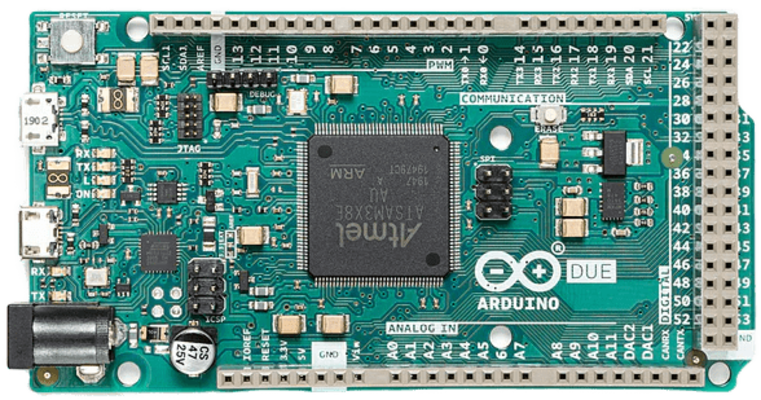
\includegraphics[height=0.49\textwidth]{images/arduino.png}
        \subcaption{Arduino Due.}
    \end{subfigure}
    \hfill \hfill \hfill
    \begin{subfigure}[m]{0.36\textwidth}
        \centering
        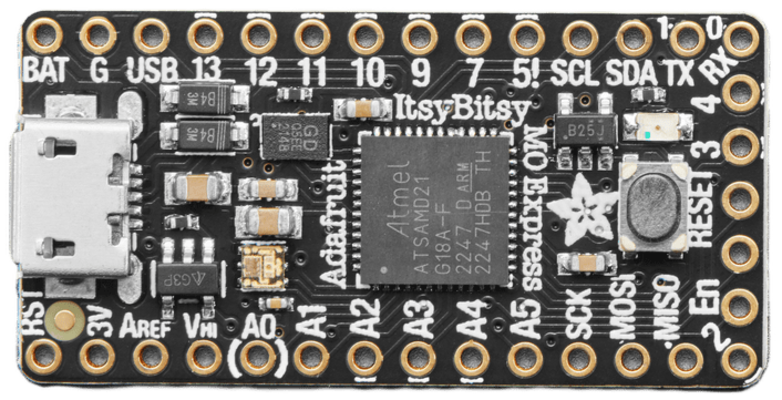
\includegraphics[height=0.40\textwidth]{images/adafruit.png}
        \subcaption{Adafruit ItsyBitsy M0 Express.}
    \end{subfigure}
    \hfill
    \begin{subfigure}[m]{0.30\textwidth}
    \centering
        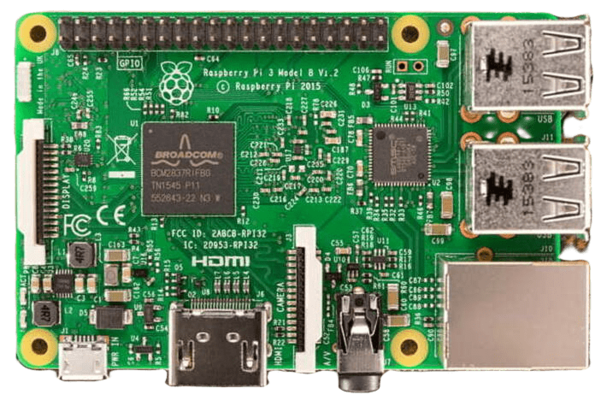
\includegraphics[height=0.48\textwidth]{images/raspberry.png}
        \subcaption{Raspberry Pi 3 Model B.}
    \end{subfigure}
\end{figure}

\end{frame}

%=======================================================================

\begin{frame}{Compilazione e raccolta dati}

\begin{center}
    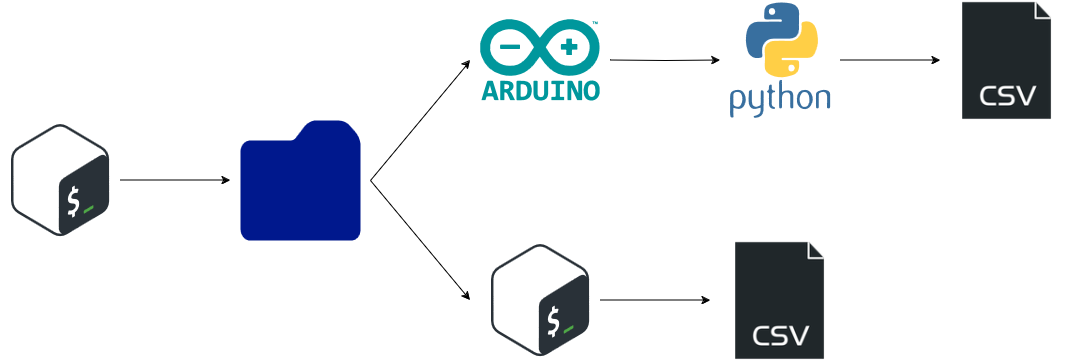
\includegraphics[height=0.3\textwidth]{images/workflow.png}
\end{center}

\end{frame}


\section{Testing e analisi dei risultati}

%=======================================================================

\begin{frame}{Sotto-famiglie di ASCON}
    \begin{columns}

    \begin{column}{0.28\textwidth}

    \begin{block}{Hash}
        \begin{center}
            Algoritmi hash e XOF
        \end{center}
    \end{block}

    \end{column}
    
    \begin{column}{0.38\textwidth}

    \begin{block}{AEAD}
        \begin{center}
            Algoritmi di cifratura autenticata
        \end{center}
    \end{block}

    \end{column}

    \begin{column}{0.28\textwidth}

    \begin{block}{Auth}
        \begin{center}
            Algoritmi MAC e PRF
        \end{center}
    \end{block}

    \end{column}

    \end{columns}

    \vspace{14pt}

    \begin{center}
        Per ogni sotto-famiglia qui sopra è stato scelto un algoritmo e analizzato per tempi di esecuzione e spazio utilizzato; i risultati di tale analisi sono inseriti in due tipi di grafico
    \end{center}

    \begin{columns}

    \begin{column}{0.5\textwidth}
        \begin{block}{Tempi di esecuzione}
            \begin{center}
                Contiene gruppi di tre colonne che rappresentano, per ogni implementazione, le misurazioni minima, media e massima
            \end{center}
        \end{block}
    \end{column}

    \begin{column}{0.5\textwidth}
        \begin{block}{Spazio utilizzato}
            \begin{center}
                Contiene una sola colonna per ogni implementazione e ognuna indica la dimensione dell'eseguibile
            \end{center}
        \end{block}
    \end{column}
        
    \end{columns}

\end{frame}

%=======================================================================

\begin{frame}{AEAD: ascon128a}

    \begin{center}
        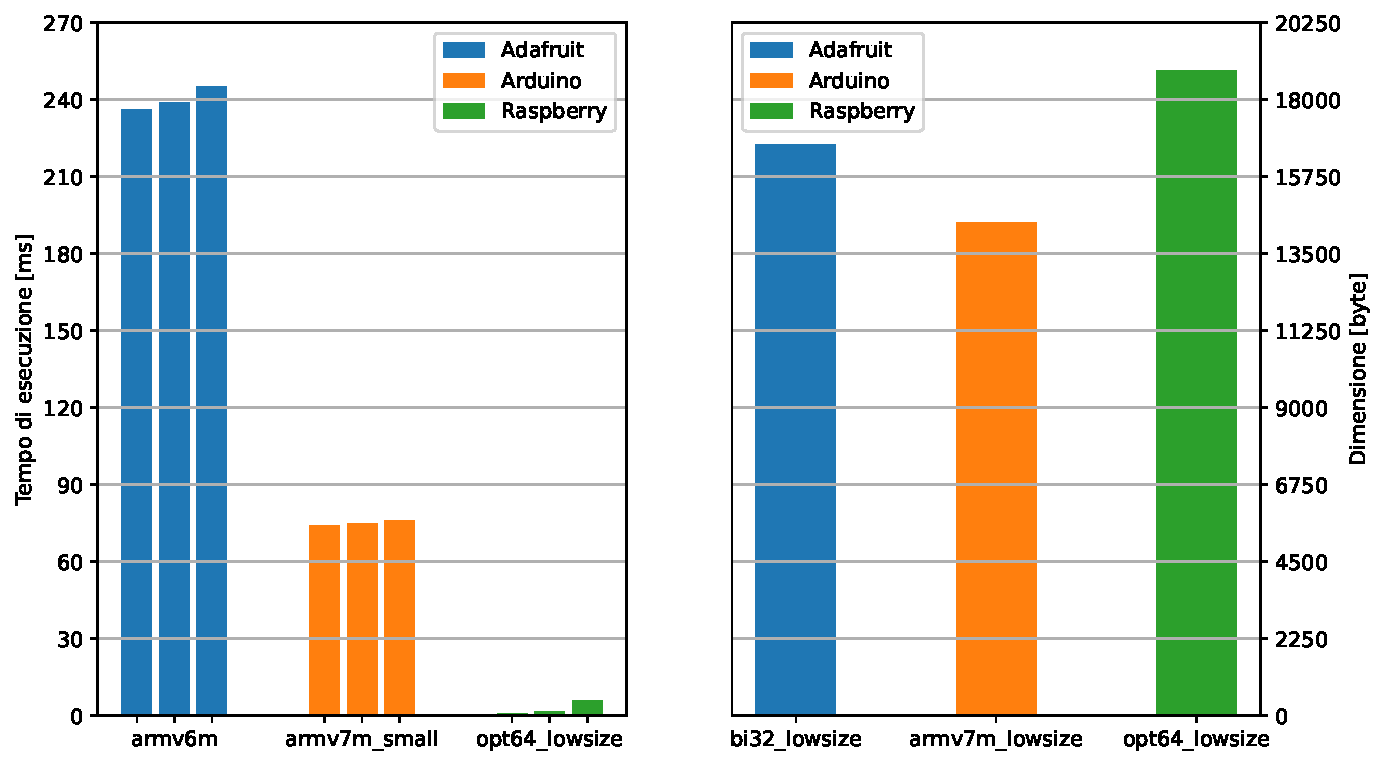
\includegraphics[height=0.40\textwidth]{images/analysis/aead.pdf}
    \end{center}
    
\end{frame}

%=======================================================================

\begin{frame}{Hash: asconhasha}

    \begin{center}
        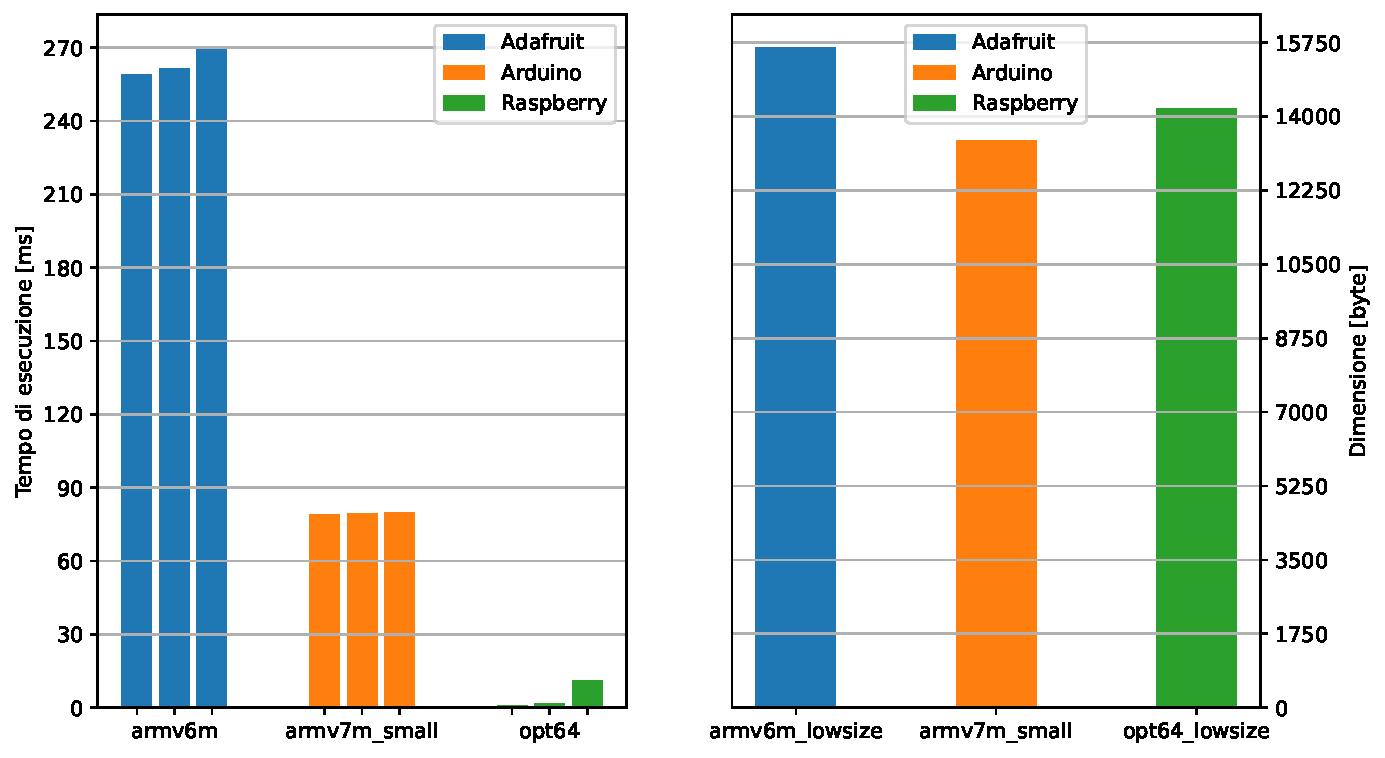
\includegraphics[height=0.40\textwidth]{images/analysis/hash.pdf}
    \end{center}
    
\end{frame}

%=======================================================================

\begin{frame}{Auth: asconmaca}

    \begin{center}
        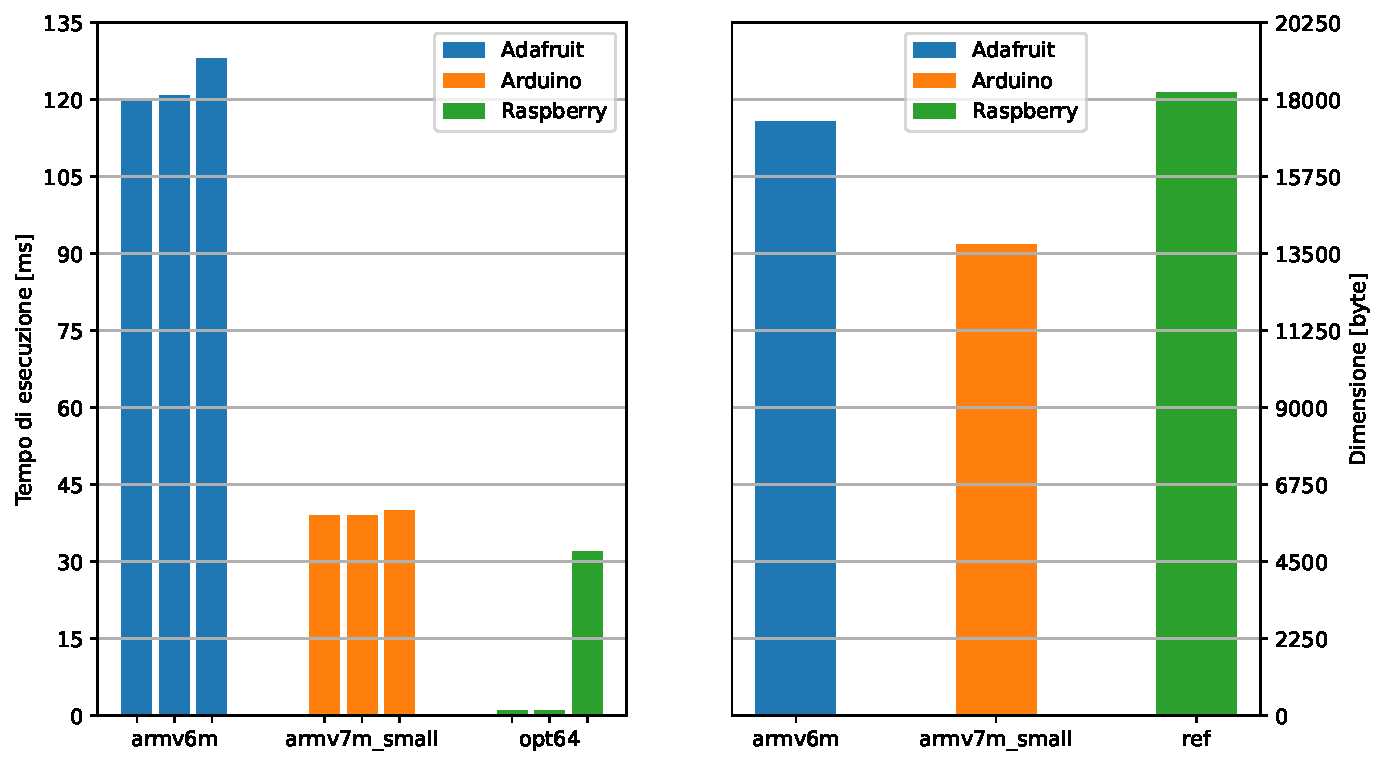
\includegraphics[height=0.40\textwidth]{images/analysis/auth.pdf}
    \end{center}
    
\end{frame}

%=======================================================================

\begin{frame}{Migliori implementazioni per ogni dispositivo}

    \begin{table}
        \centering
        \begin{tblr}{
            cells = {c},
            cell{1}{1} = {r=2}{},
            cell{1}{2} = {c=3}{},
            vlines,
            hline{1,3-6} = {-}{},
            hline{2} = {2-4}{},
        }
            \textbf{Dispositivo} & \textbf{Ottimizzazione proposta} & & \\
            & \textbf{Tempo} & \textbf{Spazio} & \textbf{Ibrida} \\
            \textbf{Adafruit} & \texttt{armv6m} & \texttt{lowsize} & \texttt{armv6m} \\
            \textbf{Arduino} & \texttt{armv7m\_small} & \texttt{armv7m\_small} & \texttt{armv7m\_small} \\
            \textbf{Raspberry} & \texttt{opt64} & \texttt{opt64\_lowsize} & \texttt{opt64}
        \end{tblr}
    \end{table}

\end{frame}


\chapter{Conclusioni}

\section{Risultati ottenuti}

Osservando i risultati presentati nel \rif[Capitolo]{ch:test_analysis}, la board RaspberryPi è risultata la migliore. Questo risultato era abbastanza prevedibile dal momento che la potenza del processore della board influisce in maniera consistente sui tempi di esecuzione ottenuti. RaspberryPi, infatti, ha una frequenza di clock 25 volte superiore alla board Adafruit e 12.5 volte superiore a quella di Arduino e questo si ripercuote sui risultati osservati sperimentalmente. \\

\noindent Tra le due board prive di sistema operativo, la migliore è stata quella di Arduino. In questo caso, anche se il processore installato ha una frequenza di clock doppia rispetto a quello di Adafruit, questo ``fattore due'' non si riflette appieno sui tempi di esecuzione. Infatti, la board Adafruit è 1.5 volte più lenta rispetto alla board Arduino. \\

\noindent I risultati ottenuti mostrano come la famiglia ASCON sia molto veloce e occupi una quantità di spazio ridotta su tutte le board testate. Questi due caratteristiche le hanno consentito di vincere sulla concorrenza e candidarsi come la miglior famiglia di cifrari presente al processo di standardizzazione del NIST.

\section{Sviluppi futuri}

I principali sviluppi futuri si muoveranno in quattro direzioni:
\begin{enumerate}[label=\Roman*.]
    \item \textbf{Raccolta dati}: la fase di testing di tutti gli algoritmi presentati comprenderà l'analisi dei cicli della CPU tramite alcuni file di test forniti da ASCON nel loro repository Github\cite{github};
    \item \textbf{Board}: la fase di testing riguarderà altri dispositivi IoT. Infatti, il testing non è avvenuto su alcune architetture – tra le quali:
    \begin{itemize}
        \item \texttt{ARMv6} e \texttt{ARM neon} per quanto riguarda le architetture ARM;
        \item \texttt{ESP32} a 32 bit;
        \item \texttt{AVX512} a 320 bit;
        \item \texttt{AVR} a 8 bit;
        \item \texttt{RV32I} a 32 bit;
        \item \texttt{RV32B} a 32 bit.
    \end{itemize}
    \item \textbf{Grandezze di plaintext}: la fase di testing verrà estesa a grandezze di plaintext maggiori, come file che codificano immagini o video;
    \item \textbf{Testing automatico}: la fase di testing verrà resa automatica, realizzando degli script che vadano a testare in sequenza i vari algoritmi usando, ad esempio, l'Arduino IDE dal terminale e non tramite la GUI.
\end{enumerate}


% ==================///==================///==================///
% ==================/// END PRESENTATION
% ==================///==================///==================///

\backmatter[notitle]

\end{document}
